\documentclass[12pt]{article}

\usepackage[dutch]{babel}
\usepackage{a4wide}
\usepackage{amsmath}
\usepackage{enumerate}
\usepackage{eurosym}
\usepackage{url}
\usepackage{graphicx}

\author{Jos Bonsink \& Mustafa Karaalioglu}

\begin{document}

\title{Project verslag - Project Thunder}
\maketitle

\section{Abstract}

\section{Inleiding}
Enkele groepen hadden besloten met robots te gaan werken. Hierbij was het nodig om realtime de lokale posities van de robots te kunnen bepalen. Tegenwoordig wordt positiebepaling voornamelijk gedaan met behulp van GPS. Echter, is dit niet overal beschikbaar. Tevens is GPS slechts nauwkeurig tot op enkele meters. GPS is dus niet geschikt voor positiebepaling in kleine ruimtes. Andere groepen kozen ervoor om gebruik te maken van \textit{image vision} waar de robots altijd in beeld moet zijn. Dit artikel onderzoekt de mogelijkheden om realtime \cite{stankovic1988misconceptions} posities akoestisch te bepalen.

Er is reeds onderzoek geweest naar de applicatie van geluid om positie te bepalen. Enzo Mumolo, Massimiliano Nolich en Gianni Vercelli hadden een algoritme ontwikkeld voor realtime lokalisatie voor het gebruik van een microfoonarray in re\"ele omstandigheden. Zij haalden een precisie van ongeveer 20 cm voor 90\% van alle gevallen in luidruchtige omstandigheden \cite{mumolo2003algorithms}. Een microfoonarray plaatsen op een robot is duur en log. Er is ook onderzoek geweest naar goedkopere oplossingen zoals een telefoon. 

Microsoft Asia had onderzoek gepleegd naar het gebruik van telefoons om afstanden te bepalen. Ze hadden een algoritme ontwikkeld dat tot een paar centimeter precies was in stille omgevingen \cite{peng2007beepbeep}. Vervolgonderzoek breidde dit uit tot volledige positiebepaling met behulp van geluid en andere sensoren zoals een gyroscoop. Zij behaalden een resolutie van 13.9 cm voor 90\% van de gevallen \cite{qiu2011feasibility}.

Zou dit preciezer kunnen? Hoe precies kan er realtime een Android-apparaat akoestisch gelokaliseerd worden? De verwachting is dat een resolutie van 10 cm te behalen moet zijn. Dit is gebaseerd op de volgende feiten: de samplerate van een microfoon is 44100 Hz, de geluidssnelheid is 340 meter per seconde, een piepgeluid kan binnen 25 samples worden herkend.

Er zal een Android-applicatie worden ontwikkeld waarin realtime piepgeluiden gegenereerd en gedetecteerd kunnen worden met een resolutie van 25 samples. Het artikel is als volgt ingedeeld: paragraaf \ref{sec:materialen} beschrijft de gebruikte materialen en ontwikkelde methoden om realtime accurate akoestische lokalisatie uit te voeren, paragraaf \ref{sec:discussie} worden de resultaten getoond in paragraaf \ref{sec:resultaten} ge\"evalueerd en worden enkele conclusies getrokken.

\section{Materialen en methoden}
\label{sec:materialen}
De experimenten met de Android-applicatie werden uitgevoerd op HTC Desire C telefoons met Android 4.0.2. Om positiebepaling mogelijk te maken met deze telefoons moesten er drie problemen worden opgelost: Bluetooth communicatie, audio detectie en afstandsmeting.

\subsection{Bluetooth}
Er zijn minstens drie Android-apparaten nodig om lokaal de positie van \'e\'en Android-apparaat te kunnen bepalen. De benodigde communicatie verliep via een peer-to-peer \cite{schollmeier2001definition} netwerk van Bluetooth \cite{haartsen2000bluetooth} verbindingen.

Alle deelnemende apparaten moesten op \textit{Bluetooth Discoverable} worden gezet voor een oneindige periode. Zoals in figuur is getoond, startte het proces bij \'e\'en node. Deze zou zoeken naar naburige Bluetooth apparaten met het Bluetooth Discovery proces. Dit proces werd telkens gestopt wanneer er \'e\'en apparaat werd gevonden. Vervolgens werd er geprobeerd met dit apparaat te verbinden, in figuur ge\"ilustreerd als de groene telefoon. Als dit mislukte, werd Bluetooth Discovery opnieuw opgestart.

Indien het verbinden van beide apparaten was geslaagd, werd Bluetooth Discoverable uitgezet. De laatst toegevoegde node ging zoeken naar nieuwe toevoegingen voor het netwerk. Dit proces herhaalde zich totdat er na een aantal Bluetooth Discoveries geen nieuwe apparaten waren gevonden. Hierna was het dus niet meer mogelijk om het netwerk uit te breiden. Alle nodes in het netwerk waren niet meer Discoverable.

Elke nieuwe node in het netwerk ontvangt van zijn \textit{parent} een lijst met de reeds bekende mac-adressen. De node voegt zijn eigen mac-adres aan deze lijst toe. Vervolgens stuurt hij zijn eigen mac-adres naar zijn parent, die dit adres aan zijn eigen lijst toevoegt. Het mac-adres propageert door het netwerk totdat het mac-adres bij de root node is terechtgekomen. Een lijst van alle mac-adressen is op elke apparaat beschikbaar. 

\subsection{Audio detectie}
Voor het realtime detecteren van piepgeluiden moest er constant geluid opgenomen \'en geanalyseerd worden. De audiohardware bufferde continu een halve seconde aan audio. In een aparte thread werden er steeds twintig samples uit deze buffer opgehaald. Op deze samples werd een Fast Fourier Transformatie(FFT) \cite{bracewell1986fourier} toegepast. Hiermee werd het geluidssignaal als functie van tijd omgezet naar een complexe functie van amplitude en fase als functie van frequentie. 

De gegenereerde piepgeluiden bestonden uit een sinuso\"ide met een frequentie van $8820$ Hz. Na de FFT werd de lengte van het complexe getal corresponderend met de frequentie van het piepgeluid vergeleken met een drempelwaarde. Wanneer de lengte de drempelwaarde overschreed, werd het geluid herkend als een piep.

\subsection{Afstandsmeting}
De afstand tussen twee Android-apparaten werd bepaald door het tijdsverschil tussen het verzenden en ontvangen van gegenereerde piepgeluiden te meten. Uit de eerder genoemde lijst van mac-adressen in het Bluetooth-netwerk werden een \textit{master} en \textit{slave} uitgekozen aan de hand van de volgorde van de lijst. De master verzocht via Bluetooth de slave te antwoorden op zijn piepgeluid. Na bevestiging van de slave, speelde de master een piepgeluid af.

Het tijdsverschil tussen het versturen en ontvangen van piepgeluiden kon worden gemeten door het aantal samples tussen twee piepgeluiden te gebruiken. Het twee keer achterelkaar detecteren van hetzelfde piepgeluid, werd voorkomen door een korte periode na een detectie niks te detecteren. De looptijd kon exact worden verkregen door te corrigeren voor de verwerkingstijd die nodig is bij het afspelen van geluid. Voor de master werd het aantal samples tussen de detectie van zijn eigen piep en dat van de respons gemeten. Bij de slave werd het verschil gemeten tussen de detectie van het eerste piepgeluid en dat van zichzelf. Dit verschil werd via Bluetooth naar de master verstuurd. De master trok deze waarde af van de gemeten totaal aantal samples totdat een andere piep werd gehoord. Aan de hand van de samplerate (44100Hz) kon de tijdsduur worden bepaald, hiermee kon vervolgens de afstand worden berekend.

\section{Resultaten}
\label{sec:resultaten}
In figuur 1 en 2 
\begin{figure}[h]
\centering
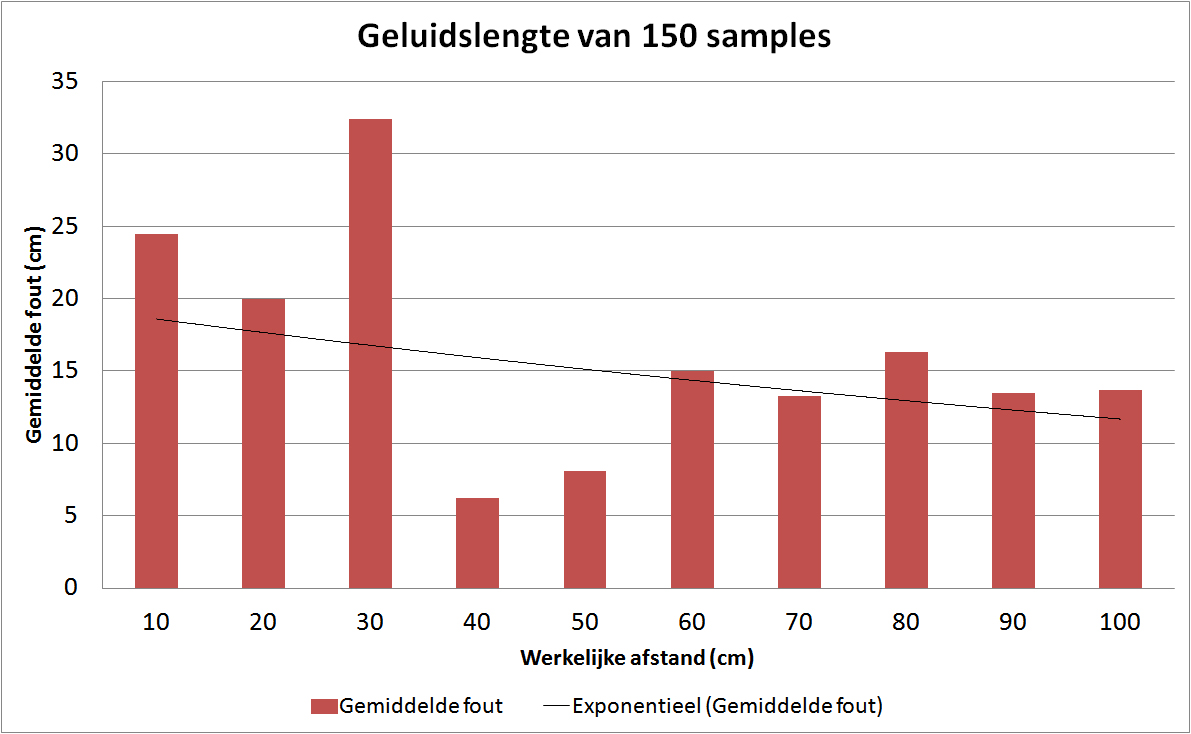
\includegraphics[scale=0.4]{150-samples}
\caption{Gemiddelde fout bij piepgeluid met geluidslengte van 150 samples.}
\end{figure}

\begin{figure}[h]
\centering
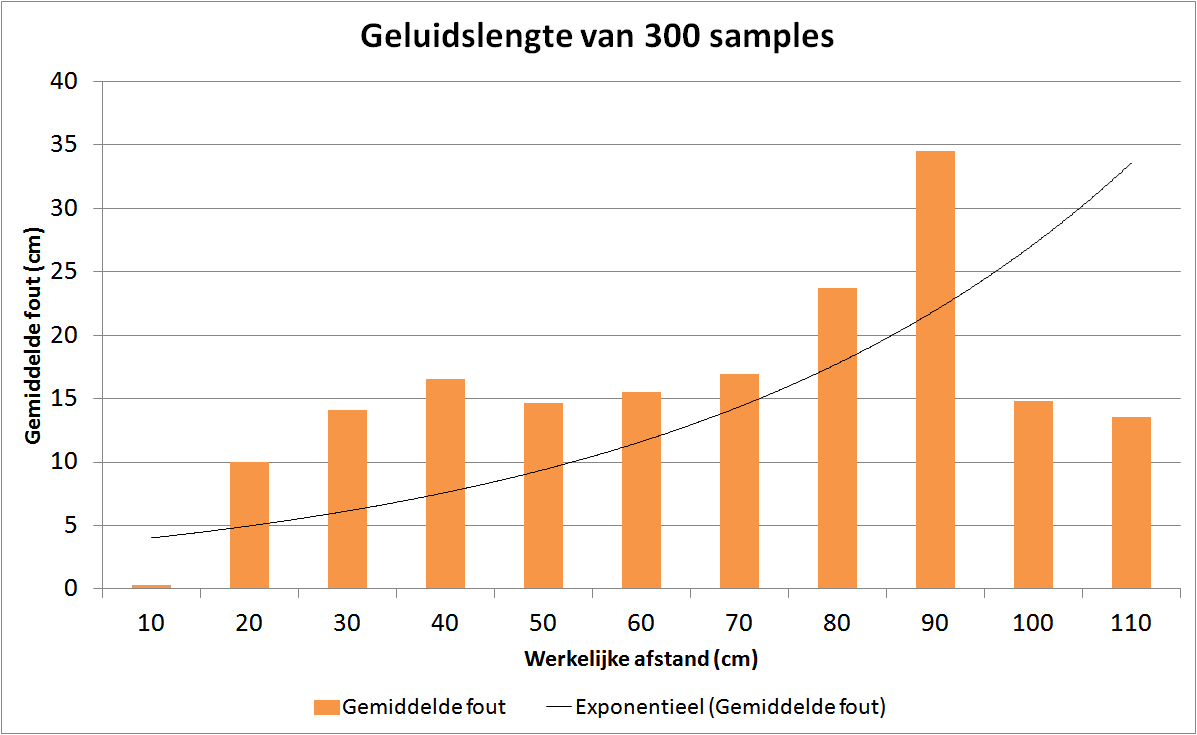
\includegraphics[scale=0.4]{300-samples}
\caption{Gemiddelde fout bij piepgeluid met geluidslengte van 150 samples.}
\end{figure}

\section{Discussie}
\label{sec:discussie}

Het meetproces is te fragiel gebleken en is niet geschikt voor nauwkeurige positie bepaling. Uit figuur blijkt dat 25\% van de afstandsmetingen mislukken, dit kan worden veroorzaakt doordat een piepgeluid 

kunnen deze herkend en herhaald worden. Dit levert een derde meer bruikbare metingen op. In voorgaand onderzoek waren in 90\% van de gevallen afstanden tot 13.9 cm nauwkeurig te meten. De gebruikte materialen in dit onderzoek waren niet toereikend om tot dezelfde of betere resultaten gekomen, zoals gebleken is in figuur .

\section{Nawoord}
\label{sec:nawoord}
Mustafa had zich tijdens het project gericht op het audio gedeelte en Jos op het Bluetooth gedeelte.


\bibliographystyle{plain}
\bibliography{refs}

\end{document}


